% ============================================================
% Projection-pipeline diagram: raw CICIoT2023 -> episode trajectory
% Compile with:  pdflatex projection_pipeline.tex
% Output:        projection_pipeline.pdf
% ============================================================
\documentclass[border=4pt]{standalone}
\usepackage{tikz}
\usetikzlibrary{shapes.geometric, arrows.meta, positioning, fit, backgrounds, calc}
\usepackage{amsmath, amssymb}

% ---- colour palette (matches architecture_diagram.tex) -------
\definecolor{colRaw}{RGB}{220,235,245}      % light blue  -- raw data
\definecolor{colProc}{RGB}{220,245,220}     % light green -- processed
\definecolor{colEnv}{RGB}{245,235,215}      % light amber -- environment
\definecolor{colBorder}{RGB}{80,100,120}
\definecolor{colArrow}{RGB}{60,80,100}

\tikzset{
  box/.style={
    rectangle, rounded corners=3pt,
    draw=colBorder, line width=0.7pt,
    text centered, font=\small,
    inner sep=5pt, minimum height=1.8em
  },
  rawBox/.style={box, fill=colRaw, minimum width=3.4cm, align=center},
  procBox/.style={box, fill=colProc, minimum width=3.4cm, align=center},
  envBox/.style={box, fill=colEnv, minimum width=3.4cm, align=center},
  groupLabel/.style={font=\small\bfseries, text=colBorder},
  arr/.style={-{Stealth[length=5pt]}, line width=0.8pt, color=colArrow},
  arrL/.style={arr, font=\footnotesize, text=colBorder},
}

\begin{document}
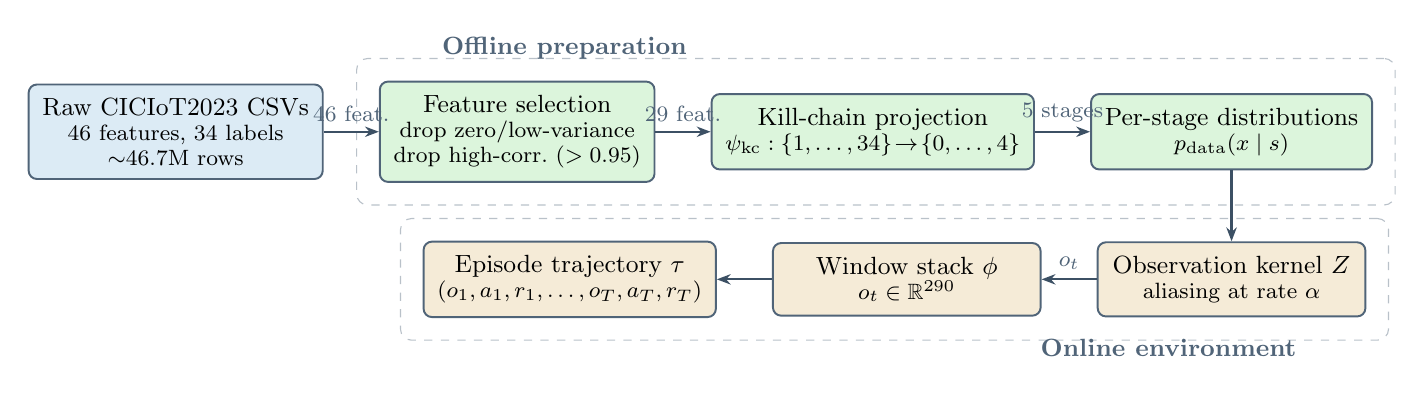
\begin{tikzpicture}[node distance=0.55cm and 0.7cm]

% ---- Nodes (left-to-right pipeline) ---------------------------
\node[rawBox] (raw) {Raw CICIoT2023 CSVs\\[-2pt]\footnotesize $46$ features, $34$ labels\\[-2pt]\footnotesize $\sim$46.7M rows};

\node[procBox, right=of raw] (fsel) {Feature selection\\[-2pt]\footnotesize drop zero/low-variance\\[-2pt]\footnotesize drop high-corr.\ ($>0.95$)};

\node[procBox, right=of fsel] (proj) {Kill-chain projection\\[-2pt]\footnotesize $\psi_{\text{kc}}:\{1,\dots,34\}\!\to\!\{0,\dots,4\}$};

\node[procBox, right=of proj] (dist) {Per-stage distributions\\[-2pt]\footnotesize $p_{\text{data}}(x\mid s)$};

\node[envBox, below=0.9cm of dist] (kernel) {Observation kernel $Z$\\[-2pt]\footnotesize aliasing at rate $\alpha$};

\node[envBox, left=of kernel] (stack) {Window stack $\phi$\\[-2pt]\footnotesize $o_t\in\mathbb{R}^{290}$};

\node[envBox, left=of stack] (traj) {Episode trajectory $\tau$\\[-2pt]\footnotesize $(o_1,a_1,r_1,\dots,o_T,a_T,r_T)$};

% ---- Arrows ----------------------------------------------------
\draw[arr] (raw) -- node[arrL, above]{46 feat.} (fsel);
\draw[arr] (fsel) -- node[arrL, above]{29 feat.} (proj);
\draw[arr] (proj) -- node[arrL, above]{5 stages} (dist);
\draw[arr] (dist) -- (kernel);
\draw[arr] (kernel) -- node[arrL, above]{$o_t$} (stack);
\draw[arr] (stack) -- (traj);

% ---- Group labels ---------------------------------------------
\node[groupLabel, above=0.15cm of fsel, xshift=0.6cm] {Offline preparation};
\node[groupLabel, below=0.15cm of kernel, xshift=-0.8cm] {Online environment};

% ---- Background groups ----------------------------------------
\begin{scope}[on background layer]
  \node[fit=(fsel)(proj)(dist), draw=colBorder!40, dashed, rounded corners, inner sep=8pt] (gProc) {};
  \node[fit=(kernel)(stack)(traj), draw=colBorder!40, dashed, rounded corners, inner sep=8pt] (gEnv) {};
\end{scope}

\end{tikzpicture}
\end{document}
